%%
%% ACM sigconf survey report generated using template.tex
%%
\documentclass[sigconf,nonacm]{acmart}

\usepackage{tabularx}
\usepackage{array}
\usepackage{tikz}
\usetikzlibrary{positioning,arrows.meta,calc}

\newcolumntype{Y}{>{\raggedright\arraybackslash}X}
\newcolumntype{C}{>{\centering\arraybackslash}X}

\settopmatter{printacmref=false}
\renewcommand\footnotetextcopyrightpermission[1]{}
\pagestyle{plain}

\title[Safeguarding Enterprise AI Agents (2020--2026)]{Safeguarding Enterprise AI Agents:\\
A Survey of Data Connectors, Deterministic Controls, and Governed Business Actions (2020--2026)}

\author{Author Name}
\authornote{Corresponding author.}
\email{author@enterprise-ai-research.org}
\affiliation{%
  \institution{Department of Computer Science \& Systems Engineering}
  \city{San Francisco}
  \state{California}
  \country{USA}
}

\renewcommand{\shortauthors}{Author Name}

\begin{abstract}
\noindent Modern enterprises are rapidly transitioning from passive, conversational Large Language Model (LLM) assistants to autonomous \emph{agentic systems}. These agents actively ingest corporate data from enterprise resource planning (ERP) and customer relationship management (CRM) systems, synthesize plans, invoke internal and external APIs, and execute consequential business actions such as customer outreach, financial approvals, and data mutations. In this agentic paradigm, a model error no longer merely outputs an inaccurate sentence; it triggers an unauthorized, unrecoverable, or costly \emph{business action}. 

  This survey provides a comprehensive review of the emerging literature (2020--2026) and industrial practice on safeguarding enterprise AI agents. We synthesize existing work into an end-to-end reference architecture spanning the entire data-to-action pipeline: enterprise data sources $\rightarrow$ ingestion connectors $\rightarrow$ curated data stores $\rightarrow$ safeguarded AI agents $\rightarrow$ controlled tools $\rightarrow$ governed business actions. We structure the taxonomy of safeguards around three foundational research questions: can the agent \emph{know} the right thing, \emph{decide} the right thing, and \emph{do} the right thing safely? 

  Crucially, we argue that AI safeguarding is fundamentally a \emph{systems-engineering challenge} rather than a purely model-centric alignment problem. We establish the \emph{Determinism Principle}---reliable software code, rather than stochastic language models, must strictly govern authorization, thresholds, schemas, action quotas, and state transitions. Grounding our survey in concrete production implementations, we analyze tenant-isolated vector retrieval, hybrid mathematical-probabilistic scoring, durable Claim-Before-Send action ledgers, multi-tier budget controls, and stateful human-in-the-loop interrupts. Finally, we provide a detailed comparative analysis of modern agent frameworks, an end-to-end case study of a four-stage lead-nurturing pipeline, and an agenda highlighting critical research gaps in verifiable agent safety.
\end{abstract}

\begin{CCSXML}
<ccs2012>
 <concept>
  <concept_id>10002978.10003022</concept_id>
  <concept_desc>Security and privacy~Software security engineering</concept_desc>
  <concept_significance>500</concept_significance>
 </concept>
 <concept>
  <concept_id>10010147.10010178.10010199</concept_id>
  <concept_desc>Computing methodologies~Multi-agent systems</concept_desc>
  <concept_significance>500</concept_significance>
 </concept>
 <concept>
  <concept_id>10010520.10010575</concept_id>
  <concept_desc>Computer systems organization~Reliable systems</concept_desc>
  <concept_significance>300</concept_significance>
 </concept>
</ccs2012>
\end{CCSXML}

\ccsdesc[500]{Security and privacy~Software security engineering}
\ccsdesc[500]{Computing methodologies~Multi-agent systems}
\ccsdesc[300]{Computer systems organization~Reliable systems}

\keywords{AI Agents, Enterprise Safeguarding, Data Connectors, Determinism Principle, Prompt Injection Defense, Action Idempotency, Systems Governance}

\maketitle

\section{Introduction}
\label{sec:intro}
Over the past five years, natural language processing has undergone a profound paradigm shift. The introduction of large-scale pretrained transformers and instruction tuning \cite{ouyang2022instructgpt,vaswani2017attention} initially enabled read-only enterprise assistants designed for search, summarization, and interactive Q\&A \cite{lewis2020rag,gao2023ragsurvey}. While transformative, these early systems were fundamentally informational: the output of the model was consumed by a human, who retained exclusive agency over downstream corporate execution.

Current enterprise deployments have aggressively moved toward \emph{autonomous agentic systems} \cite{wang2024agents,yao2023react,schick2023toolformer}. In an agentic architecture, the language model is not simply an interactive text generator; it serves as a central reasoning engine in an autonomous loop. The agent decomposes high-level human objectives, generates intermediate execution plans, retrieves semi-structured context from corporate databases, selects external tools from allow-listed APIs, and executes state-mutating actions across enterprise resource planning (ERP), customer relationship management (CRM), marketing automation, and financial ledger systems \cite{anthropic2024effective,mialon2023augmented}.

\subsection{The Expanded Enterprise Blast Radius}
This transition from passive drafting to autonomous action execution fundamentally magnifies every known vulnerability of foundation models. In an interactive chatbot, a hallucination \cite{ji2023hallucination} merely misinforms the reader; in an agentic procurement workflow, a hallucination translates into an erroneous purchase order, an unvetted vendor agreement, or an unintended legal commitment. Similarly, while prompt injection in a conversational assistant might produce an offensive response \cite{perez2022ignore}, an indirect prompt injection embedded within a customer e-mail or CRM record can hijack an agent's reasoning loop, prompting it to exfiltrate proprietary customer data or initiate unauthorized financial transfers \cite{greshake2023indirect,zhan2024injecagent}.

The fundamental threat in enterprise deployments is defined by the \emph{Lethal Trifecta} \cite{willison2025trifecta}:
\begin{enumerate}[leftmargin=*]
  \item \textbf{Access to Private Data:} The agent is granted authenticated access to proprietary internal documents, confidential customer profiles, and financial databases.
  \item \textbf{Exposure to Untrusted Input:} The agent processes unverified third-party content, including inbound sales inquiries, customer service tickets, vendor proposals, and web crawl results.
  \item \textbf{Ability to Execute External Actions:} The agent is equipped with tool capabilities to transmit e-mails, mutate records, invoke third-party APIs, and schedule background jobs.
\end{enumerate}
When all three properties coincide within an unconstrained probabilistic system, any compromise of the reasoning engine results in direct, irreversible corporate damage.

\subsection{The Limits of Model-Centric Safety}
Contemporary AI safety literature has heavily focused on model-centric mechanisms: reinforcement learning from human feedback (RLHF) \cite{ouyang2022instructgpt}, constitutional AI \cite{bai2022constitutional}, system-prompt guardrails \cite{rebedea2023nemo}, and auxiliary safety classifiers such as Llama Guard \cite{inan2023llamaguard}. While these methods are essential baselines, they are structurally insufficient for enterprise operations for several reasons:
\begin{itemize}[leftmargin=*]
  \item \textbf{Stochasticity and Drift:} Foundation models are inherently probabilistic. Even with temperature parameter $T=0$, minor variations in prompt formatting or floating-point non-determinism across GPU clusters can alter decision boundaries. Enterprises cannot accept non-deterministic adherence to compliance, privacy, or fiscal policies.
  \item \textbf{Data-Plane Vulnerabilities:} In enterprise workflows, the data ingested by the agent is itself the attack vector. Safety classifiers trained on conversational toxicity routinely fail to detect indirect prompt injections encoded as business jargon, base64 payloads, or subtle role-play instructions hidden within legitimate business documents \cite{debenedetti2024agentdojo,zou2023universal}.
  \item \textbf{Absence of Systems Properties:} High-level safety training cannot enforce operational software invariants such as relational least-privilege access, immutable audit logging, idempotent external writes, multi-tier budget reservation, or cryptographic credential secrecy.
\end{itemize}

\subsection{Research Position and Survey Scope}
This survey advances the thesis that \textbf{AI safeguarding is fundamentally a systems-engineering problem, not merely a model-quality problem.} The primary objective of an enterprise AI architecture is to insulate probabilistic AI reasoning with deterministic, permission-aware, and observable systems software so that model uncertainty never directly translates into an unsafe business action.

\subsection{Survey Methodology and Paper Organization}
Our review synthesizes academic literature and industrial system implementations published between 2020 and 2026, spanning agent frameworks, retrieval systems, prompt-injection defenses, and AI safety regulations. The remainder of this survey follows the standardized academic survey structure:
\begin{itemize}[leftmargin=*]
  \item \textbf{Section~\ref{sec:arch} (Background / Taxonomy):} Defines the reference pipeline architecture, failure modes across trust boundaries, and a 12-factor safeguards taxonomy (Table~1).
  \item \textbf{Section~\ref{sec:know} (Literature Review: Data Grounding):} Critically reviews connector architectures, credential encryption, multi-tenant vector stores, and anti-hallucination citations.
  \item \textbf{Section~\ref{sec:decide} (Literature Review: Deterministic Gating):} Critically reviews precondition validation, hybrid mathematical-probabilistic scoring, and defensive schema parsing.
  \item \textbf{Section~\ref{sec:do} (Literature Review: Action Execution \& Tools):} Critically reviews least privilege, Claim-Before-Send idempotency ledgers, prompt-injection defenses, and human oversight.
  \item \textbf{Section~\ref{sec:gov} (Literature Review: Governance \& Standards):} Reviews distributed tracing, 3-tier budget reservations, regression fixtures, and regulatory mappings (NIST, EU AI Act, OWASP).
  \item \textbf{Section~\ref{sec:case} (Industrial Case Study):} Demonstrates the practical end-to-end operation of these safeguards within a four-stage lead-nurturing pipeline.
  \item \textbf{Section~\ref{sec:compare} (Comparative Analysis):} Presents a side-by-side evaluation of contemporary agent frameworks against enterprise safeguarding criteria (Table~2).
  \item \textbf{Section~\ref{sec:open} (Research Gaps):} Identifies six critical unanswered research questions to guide future research proposals.
  \item \textbf{Section~\ref{sec:conclusion} (Conclusion):} Synthesizes the core findings and offers a closing perspective on verifiable enterprise agent systems.
\end{itemize}

\section{Background and Taxonomy}
\label{sec:arch}

\begin{figure*}[t]
\centering
\resizebox{0.95\textwidth}{!}{%
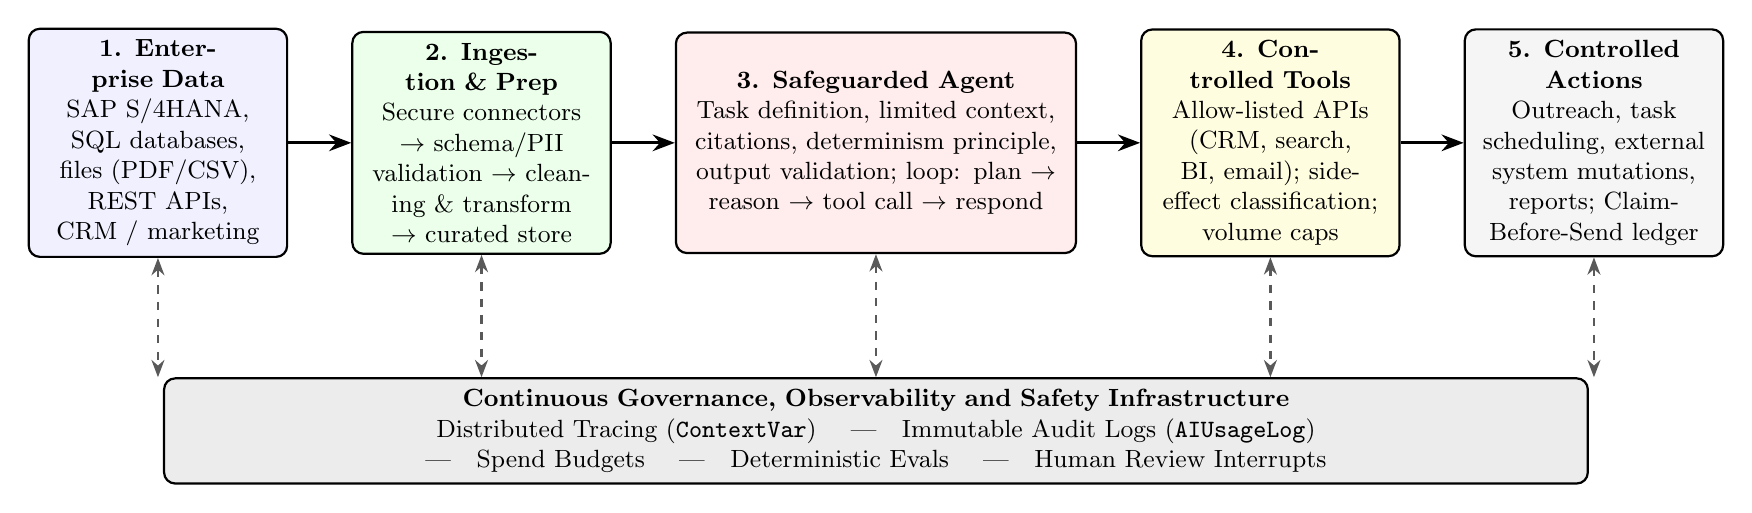
\begin{tikzpicture}[
  every node/.style={font=\small},
  box/.style={draw, rounded corners=4pt, align=center, text width=3.0cm, minimum height=2.8cm, fill=blue!6, inner sep=4pt, line width=0.8pt},
  agent/.style={draw, rounded corners=4pt, align=center, text width=4.8cm, minimum height=2.8cm, fill=red!7, inner sep=4pt, line width=0.8pt},
  gov/.style={draw, rounded corners=4pt, align=center, text width=17.8cm, minimum height=1.1cm, fill=gray!15, inner sep=4pt, line width=0.8pt},
  flow/.style={-{Stealth[length=2.8mm]}, thick, line width=1.2pt},
  ctl/.style={{Stealth[length=2.2mm]}-{Stealth[length=2.2mm]}, dashed, thick, gray!70!black}
]
\node[box] (src) {\textbf{1. Enterprise Data}\\ SAP S/4HANA, SQL databases, files (PDF/CSV), REST APIs, CRM / marketing};
\node[box, right=8mm of src, fill=green!8] (ing) {\textbf{2. Ingestion \& Prep}\\ Secure connectors $\rightarrow$ schema/PII validation $\rightarrow$ cleaning \& transform $\rightarrow$ curated store};
\node[agent, right=8mm of ing] (agt) {\textbf{3. Safeguarded Agent}\\ Task definition, limited context, citations, determinism principle, output validation; loop: plan $\rightarrow$ reason $\rightarrow$ tool call $\rightarrow$ respond};
\node[box, right=8mm of agt, fill=yellow!12] (tools) {\textbf{4. Controlled Tools}\\ Allow-listed APIs (CRM, search, BI, email); side-effect classification; volume caps};
\node[box, right=8mm of tools, fill=gray!8] (act) {\textbf{5. Controlled Actions}\\ Outreach, task scheduling, external system mutations, reports; Claim-Before-Send ledger};
\draw[flow] (src) -- (ing);
\draw[flow] (ing) -- (agt);
\draw[flow] (agt) -- (tools);
\draw[flow] (tools) -- (act);
\node[gov] (gov) at ($(src.south)!0.5!(act.south)+(0,-2.2cm)$) {\textbf{Continuous Governance, Observability and Safety Infrastructure}\\
Distributed Tracing (\texttt{ContextVar}) \quad|\quad Immutable Audit Logs (\texttt{AIUsageLog}) \quad|\quad Spend Budgets \quad|\quad Deterministic Evals \quad|\quad Human Review Interrupts};
\foreach \n in {src,ing,agt,tools,act}{\draw[ctl] (\n.south) -- (\n.south |- gov.north);}
\end{tikzpicture}}
\caption{The end-to-end Enterprise AI Safeguarding Reference Architecture. Safeguarding controls operate at ingestion, context formulation, model decision-making, tool invocation, and action dispatch, unified by a continuous governance substrate.}
\label{fig:arch}
\end{figure*}

Figure~\ref{fig:arch} illustrates the comprehensive Enterprise AI Safeguarding Reference Architecture. Rather than treating safety as an output filter applied after an LLM generates a response, safeguarding is implemented as an end-to-end architectural property distributed across five pipeline stages and supported by a continuous governance layer.

\subsection{Pipeline Stages and Trust Boundaries}
The reference architecture defines five strict trust boundaries:
\begin{enumerate}[leftmargin=*]
  \item \textbf{Enterprise Data Sources to Curated Store:} Heterogeneous enterprise data sources (relational databases, ERP systems, document repositories, SaaS applications) cannot be accessed directly by models. An ingestion layer authenticates, scrubs PII, normalizes schemas, and synchronizes records into a governed curated store.
  \item \textbf{Curated Store to Agent Context:} Raw storage is not dumped into prompts. Context assembly enforces principal-based authorization, vector similarity filtering, and strict token ceilings.
  \item \textbf{Context to Model Decision:} The reasoning loop is bounded by explicit task manifests, dependency preconditions, and deterministic business logic implemented in native code.
  \item \textbf{Decision to Tool Gateway:} Tool invocations are intercepted by software gateways that validate argument schemas, enforce allow-lists, and classify operations by their side-effect profile.
  \item \textbf{Tool Execution to External Mutation:} External side effects (e.g., e-mail transmission, financial ledger updates) are governed by durable idempotency ledgers, rate limiters, and human approval checkpoints.
\end{enumerate}

\subsection{The Threat Landscape}
Enterprise agent deployments face a dual threat landscape consisting of accidental systemic failures and deliberate adversarial attacks:
\begin{itemize}[leftmargin=*]
  \item \textbf{Indirect Prompt Injection:} Attackers embed malicious instructions within third-party documents, sales inquiries, or customer tickets \cite{greshake2023indirect,zhan2024injecagent}. When an agent ingests these texts, the model confuses data with control flow, executing the attacker's payload.
  \item \textbf{Retrieval Poisoning (PoisonedRAG):} Malicious actors inject subtly corrupted documents into corporate repositories \cite{zou2024poisonedrag}, causing RAG systems to surface inaccurate facts or biased recommendations.
  \item \textbf{Data Leakage and Training Extraction:} In multi-tenant environments, over-broad retrieval queries can return confidential documents belonging to other departments or tenants \cite{carlini2021extracting}.
  \item \textbf{Autonomous Tool Runaways:} Non-deterministic planning loops can enter infinite self-invocation cycles, repeatedly consuming API tokens, generating massive cloud bills, or spamming external partners \cite{ruan2024toolemu,yao2024taubench}.
  \item \textbf{State Corruption on Distributed Failure:} In asynchronous architectures, container crashes during external tool calls can lead to uncoordinated retries, resulting in duplicate transactions or out-of-order execution.
\end{itemize}

\subsection{The Determinism Principle}
To establish reliable software boundaries around probabilistic components, we formalize the \textbf{Determinism Principle}:

\begin{quote}
\emph{Never delegate to a probabilistic language model any decision, verification, or threshold that can be computed deterministically by standard software code.}
\end{quote}

Under this principle, responsibilities are strictly partitioned:
\begin{itemize}[leftmargin=*]
  \item \textbf{Deterministic Software Code Owns:} Identity and authentication, role-based access control (RBAC), multi-tier budget tracking, schema parsing, numerical metric clamping, rate limiting, action idempotency, and workflow state transitions.
  \item \textbf{Probabilistic Models Own:} Natural language understanding, contextual semantic extraction, unstructured text synthesis, classification refinement, and stylistic personalization.
\end{itemize}

Table~\ref{tab:safeguards} details how twelve core safeguards instantiate this principle across the entire system lifecycle.

\begin{table*}[t]
\centering
\caption{Comprehensive taxonomy of enterprise AI safeguards, theoretical foundations, threat mitigation, and systems software mechanisms.}
\label{tab:safeguards}
\footnotesize
\begin{tabularx}{\textwidth}{@{}p{2.6cm} p{1.3cm} Y Y Y@{}}
\toprule
\textbf{Safeguard} & \textbf{Question} & \textbf{What to Enforce} & \textbf{Threats Addressed} & \textbf{Concrete Systems Software Mechanism} \\
\midrule
Purpose \& Scope & Decide & Define rigid task boundaries; avoid general-purpose autonomy & Scope drift, unexpected tool use & Declarative agent manifests (\texttt{manifest.json}), dependency precondition validators (\texttt{DependencyValidator}) \\
Limit Context & Know & Inject only task-relevant, permission-appropriate records & Data exfiltration, context stuffing & Dual-tier cache/store (\texttt{ContextStore}), relational SQL predicates, hard token ceilings (3k tokens) \\
Grounding & Know & Factual claims must trace directly to verified enterprise sources & Fabricated customer/lead facts & Structured citation extraction (\texttt{chunk\_id}), deterministic entity fallback matching (\texttt{\_safe\_llm\_summary}) \\
Determinism & Decide & Execute rules, math, validation, and state machines in code & Stochastic decision drift, policy violations & Hybrid scoring ($45\%$ cosine similarity $+ 55\%$ LLM refinement at $T=0.0$), rule-based state graphs \\
Access Control & Do & Least privilege; permission to read does not imply right to act & Privilege abuse, unauthorized writes & Symmetric credential encryption at rest (\texttt{Fernet}), tenant isolation via SQL (\texttt{WHERE pd.uploaded\_by}) \\
Tool Control & Do & Allow-list and constrain tool capability surfaces & Tool poisoning, malicious parameters & Side-effect tagging (\texttt{SIDE\_EFFECT\_READ} vs.\ \texttt{IRREVERSIBLE}), hard batch volume caps (50 items) \\
Action Idempotency & Do & Guarantee durable at-most-once execution of side effects & Duplicate messages, financial re-execution & Transactional Claim-Before-Send ledger (\texttt{WorkflowSendLedger}) with SHA-1 content hashing \\
Output Validation & Decide & Validate schemas, data types, and numerical boundaries & Malformed JSON, code fence contamination & Defensive JSON parsing (\texttt{safe\_parse\_json}), type enforcement, numerical boundary clamping ($[0,100]$) \\
Human Review & Do & Enforce human oversight for high-risk or irreversible steps & Catastrophic autonomous errors & LangGraph \texttt{interrupt()}, autonomy modes (Co-pilot vs.\ Autopilot fail-safe escalation) \\
Injection Defense & Do & Treat all external text as untrusted data, never control & Indirect injection via CRM/e-mail & Instruction hierarchies, quarantined execution, capability reduction, input boundary tokenization \\
Observability & All & Capture granular distributed execution and cost traces & Unauditable model reasoning, silent drift & Asynchronous \texttt{ContextVar} tracing (\texttt{usage\_scope}), immutable \texttt{AIUsageLog}, latency profiling \\
Budget Governance & All & Prevent unbounded financial expenditure on API inference & Denial-of-wallet, runaway agent loops & Three-tier spend caps (User, Project, Team), pre-call reservations (\texttt{reserve\_budget}), HTTP 402 blocking \\
\bottomrule
\end{tabularx}
\end{table*}

\section{Literature Review: Data Grounding and Epistemology (Can the Agent Know?)}
\label{sec:know}

The first foundational challenge in safeguarding enterprise agents is epistemological: how can we guarantee that the information presented to the model is accurate, authorized, task-relevant, and resistant to adversarial manipulation?

\subsection{Ingestion, Connectors, and Cryptographic Security}
Enterprise agents rely on connectors to interface with heterogeneous storage systems, including ERP suites (SAP S/4HANA), relational databases (PostgreSQL, MySQL), semi-structured document stores (PDF, CSV, Office files), and third-party SaaS APIs (Salesforce, HubSpot, LinkedIn, Google Business). 

\paragraph{Connector lifecycle abstraction.} In production software architectures, connectors are organized into a strict class hierarchy rooted in an abstract \texttt{BaseConnector} (\texttt{backend/core/connectors/base.py}). Subclasses specialize into OAuth connectors, API-key connectors, session-based web scrapers, and stateless HTTP clients. Robust implementations enforce four distinct lifecycle phases:
\begin{enumerate}[leftmargin=*]
  \item \texttt{connect()}: Establishes network transport and validates cryptographic authentication tokens before exposing data endpoints.
  \item \texttt{health\_check()}: Executes non-mutating canary probes to verify live operational status without risking data mutation.
  \item \texttt{fetch()}: Retrieves raw payloads from authoritative upstream sources while enforcing source rate limits and exponential backoff.
  \item \texttt{\_transform()}: Sanitizes, normalizes, and extracts structured records from vendor-specific payloads, applying declarative schema validation \cite{breck2019data,schelter2018deequ}.
\end{enumerate}

\paragraph{Cryptographic secret protection.} A major vulnerability in agent deployments is the insecure storage of third-party API tokens and OAuth refresh secrets. Production safeguarding mandates authenticated symmetric encryption at rest. In \texttt{backend/core/crypto.py}, secrets stored in the database are encrypted using Fernet (AES-128 in CBC mode with an HMAC-SHA256 signature for ciphertext authentication). Values remain encrypted throughout storage and are decrypted strictly in memory upon connector instantiation. Furthermore, logging subsystems enforce string masking (e.g., \texttt{mask\_value()}) to prevent credential leakage in application telemetry.

\subsection{Curated Data Stores and Tenant Isolation}
Once ingested, enterprise data must be maintained in curated stores that preserve lineage, tenant boundaries, and access control lists.

\paragraph{Dual-tier context architecture.} In \texttt{backend/core/context.py}, context management is decoupled into a dual-tier storage system (\texttt{ContextStore}):
\begin{itemize}[leftmargin=*]
  \item \textbf{Ephemeral Tier (Redis):} Provides low-latency key-value caching with bounded time-to-live (TTL, defaulting to 7200 seconds) for transient inter-agent message passing during active workflow execution.
  \item \textbf{Persistent Tier (PostgreSQL):} An immutable, relational \texttt{AgentContext} table capturing every context assignment, agent identifier, and session payload, providing durable auditability across reboots and worker restarts.
\end{itemize}
External data ingested via connectors is wrapped with provenance tracking metadata using \texttt{store\_from\_source()}, recording the originating source URL, query string, timestamp, and ingesting principal.

\paragraph{Relational tenant isolation in vector stores.} Vector similarity search (e.g., pgvector) is the standard retrieval substrate for enterprise RAG \cite{lewis2020rag}. However, vector similarity metrics (such as cosine distance) are completely agnostic to access control policies. In a naive implementation, a semantic search for ``executive compensation'' will readily return chunks from private HR documents if those chunks are stored in the same vector index.

Production architectures enforce tenant isolation not by prompting the LLM to ignore unauthorized chunks, but by compiling mandatory relational SQL constraints directly into the similarity query (\texttt{backend/core/vector_store.py}):
\begin{equation}
\label{eq:sql_tenant}
\begin{split}
\textbf{SELECT } & \texttt{dc.chunk\_id, dc.content,} \\
& 1 - (\texttt{dc.embedding} \Leftrightarrow \texttt{:query\_embedding::vector}) \textbf{ AS } \texttt{score} \\
\textbf{FROM } & \texttt{document\_chunks dc} \\
\textbf{JOIN } & \texttt{processed\_documents pd ON dc.document\_id = pd.document\_id} \\
\textbf{WHERE } & \texttt{pd.uploaded\_by = :user\_id} \quad \textbf{AND } \texttt{pd.project\_id = :project\_id} \\
\textbf{ORDER BY } & \texttt{dc.embedding} \Leftrightarrow \texttt{:query\_embedding::vector} \\
\textbf{LIMIT } & \texttt{:top\_k;}
\end{split}
\end{equation}
By binding the requesting principal's verified identity (\texttt{:user\_id}) and project boundary (\texttt{:project\_id}) into the relational join prior to similarity sorting, cross-tenant and cross-project data leakage is rendered mathematically impossible at the database engine level.

\subsection{Context Bounding and Minimization}
A prevalent misconception in early agent literature was that expanding LLM context windows (e.g., to $10^6$ tokens) eliminates the need for retrieval filtering. In enterprise safeguarding, unbounded context expansion is actively hazardous for three reasons:
\begin{enumerate}[leftmargin=*]
  \item \textbf{Information Dispersal and Recall Degradation:} Models exhibit severe ``lost in the middle'' phenomena \cite{liu2024lost}, failing to utilize facts placed in the central third of large context windows.
  \item \textbf{Attack Surface Expansion:} Every additional document injected into context represents an additional channel for indirect prompt injection and retrieval poisoning \cite{greshake2023indirect,zou2024poisonedrag}.
  \item \textbf{Financial Inefficiency:} Quadratic or linear attention costs dramatically inflate inference latency and API expenditures.
\end{enumerate}

Accordingly, defensive retrieval systems enforce strict context minimization \cite{beurerkellner2025patterns}. In \texttt{backend/agents/document_intelligence/retrieval.py}, retrievers enforce hard chunk bounds ($\text{top\_k} \le 5$) and aggregate token ceilings ($\text{max\_tokens} \le 3000$). Documents are segmented using structural, boundary-aware chunking algorithms (\texttt{chunking.py}), and retrieved passages that exceed the token budget are deterministically truncated.

\subsection{Grounding and Anti-Hallucination Fallbacks}
Grounding mandates that all factual claims generated by an agent must be verifiable against authoritative corporate evidence. 

\paragraph{Structural citation provenance.} Rather than passing raw text blobs into prompts, retrievers construct context dictionaries that explicitly pair each passage with citation metadata:
\begin{equation}
\mathcal{C} = \left\{ \langle \text{content}_i, \text{chunk\_id}_i, \text{doc\_id}_i, \text{score}_i \rangle \right\}_{i=1}^{k}
\end{equation}
Prompts instruct the model to ground every assertion with structural citation tags citing specific chunk identifiers.

\paragraph{Deterministic entity validation.} Even with grounded context, stochastic models frequently hallucinate entity names, confusing company names mentioned in reference paragraphs. In \texttt{backend/agents/sales_helper_core.py}, the validator \texttt{\_safe\_llm\_summary()} performs deterministic post-generation inspection:
\begin{equation}
\text{Valid}(S, E) = \begin{cases}
S & \text{if } \text{Lower}(E) \subseteq \text{Lower}(S) \\
S_{\text{extractive}} & \text{otherwise}
\end{cases}
\end{equation}
where $S$ is the model's generated summary and $E$ is the authoritative entity name. If the model generates a summary that fails to reference the verified enterprise name, the probabilistic text is discarded entirely, and the system falls back to a deterministic extractive summary synthesized directly from raw document sentences.

\section{Literature Review: Deterministic Gating and Reasoning (Can the Agent Decide?)}
\label{sec:decide}

Once accurate context is established, the agent enters its reasoning and decision-making phase. Safeguarding this layer requires constraining agent autonomy within rigid operational boundaries.

\subsection{Scope Management and Dependency Gating}
General-purpose conversational assistants are inherently difficult to safeguard because their operational scope is undefined. Enterprise architectures reject general assistants in favor of specialized, single-responsibility agents (e.g., market research agents, email outreach agents, compliance audit agents) coordinated through explicit workflows \cite{anthropic2024effective}.

\paragraph{Declarative dependency validation.} In \texttt{backend/core/dependency_validator.py}, agent execution is gated by a declarative dependency validator reading configuration from \texttt{agent-dependencies.json}. Each agent manifest declares its required inputs and output artifacts. For example, an outreach agent declares:
\begin{equation}
\text{Requires}(\text{email\_outreach}) = \{ \texttt{company\_profile}, \texttt{prospect\_list} \}
\end{equation}
Prior to task scheduling, \texttt{check\_dependencies()} queries the context store to verify whether these artifacts exist. Furthermore, dependencies are scoped by project identifier (\texttt{scoped\_key(dep\_key, project\_id)}). If prerequisite data is missing or belongs to an unlinked project, the runtime halts execution deterministically, returning an actionable error code and preventing premature or hallucinated agent reasoning.

\subsection{Operationalizing the Determinism Principle: Hybrid Scoring}
The Determinism Principle dictates that core algorithmic decisions must not depend on model compliance. In lead qualification and vendor evaluation (\texttt{backend/agents/sales_helper_core.py}), this principle is realized through a \emph{hybrid mathematical-probabilistic scoring pipeline}.

\paragraph{Algorithmic pipeline.} Rather than passing an entire database of 10,000 candidate leads to an LLM and asking it to ``rank the top vendors,'' the system executes a three-phase pipeline:
\begin{enumerate}[leftmargin=*]
  \item \textbf{Deterministic Baseline Ranking:} Native vectorized code generates semantic embeddings for the requirement text $\mathbf{v}_{\text{req}}$ and all candidate company descriptions $\{\mathbf{v}_{\text{cand}, i}\}_{i=1}^{N}$. Using SciPy/NumPy, the cosine similarity is computed across all records:
  \begin{equation}
  \text{sim}(\mathbf{v}_{\text{req}}, \mathbf{v}_{\text{cand}, i}) = 1 - \frac{\mathbf{v}_{\text{req}} \cdot \mathbf{v}_{\text{cand}, i}}{\|\mathbf{v}_{\text{req}}\|_2 \|\mathbf{v}_{\text{cand}, i}\|_2}
  \end{equation}
  This mathematical baseline provides an instantaneous, cost-free, and perfectly reproducible ranking across the entire database.
  \item \textbf{Top-$k$ LLM Refinement:} Only the top-$k$ candidates (e.g., $k=100$) are extracted and formatted into a structured prompt. The language model is invoked with temperature $T=0.0$ to evaluate nuanced qualitative fit (e.g., buyer vs.\ seller intent) and generate a refined match score $S_{\text{LLM}} \in [0, 100]$.
  \item \textbf{Linear Mathematical Blending:} The final score is computed via a fixed linear combination in Python:
  \begin{equation}
  S_{\text{final}} = \text{round}\left(0.45 \times S_{\text{vector}} + 0.55 \times S_{\text{LLM}}\right)
  \end{equation}
\end{enumerate}
This hybrid architecture guarantees that broad decision boundaries are anchored in reproducible vector mathematics, reducing model hallucination risk, cutting LLM token usage by over $90\%$, and preventing stochastic model drift from corrupting core enterprise rankings.

\subsection{Defensive Output Validation and Schema Clamping}
Language models are notorious for corrupting structured outputs: they inject markdown formatting fences (\texttt{```json ... ```}), omit required schema keys, hallucinate unexpected types, or generate numbers outside allowable bounds.

\paragraph{Resilient JSON parsing.} In \texttt{backend/core/ai_client.py}, all structured completions are processed through \texttt{safe\_parse\_json()}. This utility:
\begin{itemize}[leftmargin=*]
  \item Strips markdown code blocks and regex-extracts valid JSON substrings.
  \item Enforces schema validation against expected Python dictionaries or lists.
  \item Clamps numerical outputs to valid intervals, ensuring scores cannot exceed $[0, 100]$.
  \item Replaces malformed or empty responses with safe default dictionaries rather than crashing downstream execution loops.
\end{itemize}
These deterministic checks ensure that malformed model outputs are captured and corrected at the boundary before passing to external tools.

\section{Literature Review: Controlled Action Execution and Tool Safety (Can the Agent Do?)}
\label{sec:do}

The most critical risk in agentic systems arises when the model transitions from internal reasoning to external action execution. Unconstrained tool access turns model mistakes into catastrophic enterprise incidents.

\subsection{Least Privilege and Side-Effect Classification}
Following Saltzer and Schroeder's classical principle of least privilege \cite{saltzer1975protection}, an agent must never execute tools under a shared administrative service account. Instead, tool execution must be authenticated using the scoped identity of the human operator initiating the run.

\paragraph{Side-effect taxonomy.} In \texttt{backend/agents/workflow_orchestration/graph.py}, all agent tools are categorized into an explicit side-effect taxonomy:
\begin{itemize}[leftmargin=*]
  \item \texttt{SIDE\_EFFECT\_READ}: Operations that perform internal queries, database searches, vector similarity ranking, and draft synthesis. These operations do not alter external state and are safe for automated background execution.
  \item \texttt{SIDE\_EFFECT\_IRREVERSIBLE}: Operations that reach outside platform boundaries in ways that cannot be rolled back, such as dispatching real outreach e-mails, updating production CRM records, issuing vendor payments, or modifying cloud infrastructure.
\end{itemize}
Tools declared as \texttt{SIDE\_EFFECT\_IRREVERSIBLE} are strictly forbidden from executing without explicit policy evaluation and human oversight checkpoints. Furthermore, batch-oriented tools enforce code-level volume ceilings (e.g., \texttt{\_max\_email\_recipients\_per\_stage()}, capping batches at 50 recipients).

\subsection{Action Idempotency: The Claim-Before-Send Ledger}
In distributed enterprise architectures, agent tasks execute asynchronously on worker queues (e.g., Celery with Redis brokers). In real-world networks, worker processes crash, connection timeouts occur, and message brokers replay unacknowledged tasks. If an agent task crashes after transmitting an email but before reporting success, a standard retry mechanism will re-execute the task, sending duplicate messages to external clients.

\paragraph{The Claim-Before-Send protocol.} To solve this failure mode, production platforms implement a transactional \emph{Claim-Before-Send} protocol backed by a relational database table (\texttt{WorkflowSendLedger} in \texttt{backend/models/workflow.py}). The schema enforces a compound unique constraint:
\begin{equation}
\label{eq:ledger_constraint}
\begin{split}
\text{UNIQUE}(&\text{instance\_id}, \text{stage\_id}, \\
&\text{content\_hash}, \text{recipient\_email})
\end{split}
\end{equation}

The execution protocol proceeds through five distinct transactional steps:
\begin{enumerate}[leftmargin=*]
  \item \textbf{Content Hashing:} The runtime computes a deterministic 12-character SHA-1 hash over the outreach message:
  \begin{equation}
  H = \text{SHA-1}(\text{subject} \,\|\, \text{body} \,\|\, \text{personalization\_flag})[:12]
  \end{equation}
  Hashing the content ensures that re-approving an identical message reuses the ledger, while genuinely edited copy starts a fresh audit trail.
  \item \textbf{Pre-Dispatch Claiming:} Prior to invoking the SMTP gateway or external API, the runtime atomically inserts a row into \texttt{workflow\_send\_ledger} with status \texttt{"claimed"}.
  \item \textbf{Conflict Interception:} If the row already exists (due to a prior worker execution or concurrent thread), the database engine raises an \texttt{IntegrityError}. The agent intercepts this error, flags the recipient as ``already handled,'' and skips transmission.
  \item \textbf{External Transmission:} If the claim is successful, the external dispatch is executed.
  \item \textbf{Status Confirmation:} Upon verified provider delivery, the row status is updated to \texttt{"sent"}. If a worker crashes mid-send, the row remains in \texttt{"claimed"} status; subsequent retries identify the unconfirmed claim and refuse to double-send.
\end{enumerate}
This mechanism provides mathematical guarantees of at-most-once execution semantics for irreversible external actions.

\subsection{Prompt-Injection Defense in Depth}
Indirect prompt injection through ingested customer emails or CRM notes represents the primary adversarial threat to agentic execution \cite{greshake2023indirect,debenedetti2024agentdojo}. Because single-point defenses are routinely bypassed \cite{zou2023universal}, enterprise systems implement a five-layer defense-in-depth model:
\begin{enumerate}[leftmargin=*]
  \item \textbf{Instruction Hierarchies:} Models are fine-tuned to prioritize system-level instructions over user-level or data-level inputs \cite{wallace2024hierarchy}.
  \item \textbf{Spotlighting and Delimitation:} Ingested third-party text is wrapped in unambiguous XML-style delimiters and labeled as untrusted data \cite{hines2024spotlighting}.
  \item \textbf{Architectural Quarantining (CaMeL Pattern):} Untrusted text processing is isolated within quarantined sub-agents that lack tool execution privileges \cite{debenedetti2025camel}.
  \item \textbf{Privilege Reduction:} The agent loop is structured to break the ``Lethal Trifecta'' \cite{willison2025trifecta}: agents handling untrusted external inputs are stripped of arbitrary exfiltration and write capabilities.
  \item \textbf{Action Validation \& Review:} Proposed action arguments are validated against strict business rules before execution.
\end{enumerate}

\subsection{Human-in-the-Loop and Autonomy Calibration}
Human oversight is the ultimate safeguard, but naive approval workflows introduce reviewer fatigue, leading human operators to rubber-stamp agent proposals without scrutiny. Effective safeguarding requires \emph{calibrated autonomy}.

\paragraph{Operational autonomy modes.} In \texttt{backend/agents/workflow_orchestration/graph.py}, workflows support two operational autonomy modes:
\begin{itemize}[leftmargin=*]
  \item \textbf{Co-pilot Mode:} Designed for exploratory or sensitive operations. The graph engine pauses at every node by invoking LangGraph's \texttt{interrupt()} primitive. The execution payload---containing proposed tool calls, inputs, and rationale---is serialized to storage. The human supervisor reviews the proposal and issues a resume command with an explicit action: \texttt{approve} (executes as proposed), \texttt{edit} (overrides inputs with human adjustments), or \texttt{skip} (bypasses the stage without execution).
  \item \textbf{Autopilot Mode:} Designed for routine execution. Stages declared as \texttt{SIDE\_EFFECT\_READ} proceed autonomously without human intervention.
\end{itemize}

\paragraph{Fail-safe escalation.} Crucially, Autopilot mode is not unconstrained. The runtime implements \emph{automatic fail-safe escalation} (\texttt{\_autopilot\_review\_reason()}): the engine automatically forces an \texttt{interrupt()} and yields control to a human reviewer if:
\begin{enumerate}[leftmargin=*]
  \item The pending stage declares \texttt{SIDE\_EFFECT\_IRREVERSIBLE}.
  \item The project, user, or team spend has exceeded its monthly budget cap.
  \item The stage throws an unhandled exception or validator error during execution.
\end{enumerate}
In addition, an atomic kill-switch check (\texttt{\_instance\_paused()}) is evaluated at the entry of every single state graph node, immediately halting background Celery tasks if a workflow is paused in the management UI.

\section{Literature Review: Governance, Observability, and Compliance Standards}
\label{sec:gov}

The final layer of the architecture provides continuous observability, cost control, regression evaluation, and regulatory compliance across all agents.

\subsection{Distributed Observability and Tracing}
In production agent architectures, a single high-level business workflow triggers dozens of multi-hop LLM completions, embedding calculations, and external tool calls executed across distributed worker pools. Standard HTTP request logging fails in this environment because background worker threads lack HTTP request context.

\paragraph{Context-propagated usage tracing.} In \texttt{backend/core/usage_context.py}, observability is achieved using thread-safe context variables (\texttt{contextvars.ContextVar}). The orchestration engine binds execution context through a formal scope tuple:
\begin{equation}
\label{eq:usage_scope}
\begin{split}
\sigma &= \langle \text{instance\_id}, \text{stage\_id}, \text{project\_id}, \text{user\_id} \rangle \\
\mathcal{T}_{\text{exec}} &= \text{execute}(\text{state}, \text{input} \mid \sigma) \implies \text{AIUsageLog}(\sigma, \Delta_{\text{tokens}}, \text{cost})
\end{split}
\end{equation}
Implemented via \texttt{with usage\_scope(...) : output = execute(state, final\_input)} in Python, all downstream invocations within \texttt{ai\_client.py} automatically read the active scope token. Every API call records prompt tokens, completion tokens, model name, provider, latency, and estimated cost into an immutable \texttt{AIUsageLog} database table, allowing administrators to compute real-time financial attribution per workflow stage, project, and user.

\subsection{Multi-Tier Financial Budget Governance}
Runaway autonomous loops, prompt injection loops, or recursive self-refinement algorithms can rapidly deplete API quotas and generate thousands of dollars in cloud inference costs within minutes.

\paragraph{Hierarchical budget enforcement.} In \texttt{backend/core/budget.py}, the safeguarding architecture implements multi-tier budget governance across three nested scopes:
\begin{equation}
\text{Budget Scope} \in \{ \text{User}, \text{Project}, \text{Team} \}
\end{equation}
Budgets are tracked against real-time aggregations of the \texttt{AIUsageLog} table. Systems enforce two distinct operational policies:
\begin{itemize}[leftmargin=*]
  \item \textbf{Pre-Execution Reservations:} Prior to dispatching an expensive LLM call, \texttt{reserve\_budget\_for\_call()} computes an upper-bound cost estimate based on prompt characters and requested \texttt{max\_tokens}. It places a temporary reservation lock in Redis, preventing concurrent worker tasks from overdrawing the budget pool.
  \item \textbf{Hard Blocking Gate:} When a budget configured with a \texttt{"block"} policy is exhausted ($S \ge \text{Limit}$), \texttt{enforce\_budget()} halts execution and raises a \texttt{BudgetExceeded} exception. The API gateway translates this into an HTTP 402 Payment Required response, immediately terminating downstream model dispatch.
\end{itemize}

\subsection{Deterministic Regression Evaluation}
Because foundation models are updated asynchronously by upstream providers (e.g., silent checkpoint updates in hosted proprietary APIs), an agent prompt that worked reliably yesterday may suffer catastrophic drift today. 

\paragraph{Limitations of LLM-as-a-judge.} Many commercial frameworks advocate evaluating agents using ``LLM-as-a-judge'' architectures \cite{zheng2023judge} or synthetic evaluation metrics such as RAGAS \cite{es2024ragas}. In enterprise environments, LLM judges introduce severe vulnerabilities: they are non-deterministic, exhibit position and length biases, consume significant API budgets, and can be fooled by adversarial model outputs that mimic polite, helpful responses \cite{zheng2023judge}.

\paragraph{Deterministic fixture testing.} Production safeguarding mandates deterministic regression test suites. In \texttt{backend/eval/}, continuous integration pipelines maintain fixed YAML test fixtures (\texttt{fixtures/*.yaml}) capturing real enterprise input/output pairs across all LLM-calling endpoints. In \texttt{eval/scoring.py}, outputs are judged using deterministic software assertions:
\begin{itemize}[leftmargin=*]
  \item Case-insensitive keyword presence checks (\texttt{check\_keywords()}).
  \item Mandatory JSON schema and key presence verification (\texttt{check\_json\_keys()}).
  \item Structural numerical bound validation.
\end{itemize}
These deterministic gates run automatically in CI/CD pipelines, flagging behavioral regressions and cost spikes without introducing judge variance.

\subsection{Mapping to Regulatory and Industry Standards}
Enterprise AI safeguards must align with emerging global regulatory frameworks:
\begin{itemize}[leftmargin=*]
  \item \textbf{NIST AI Risk Management Framework (AI RMF 1.0) \cite{nist2023airmf}:} The four NIST functions map directly to our architecture: \emph{Govern} maps to multi-tier budget controls and access authorization; \emph{Map} maps to declarative task manifests and scope validation; \emph{Measure} maps to continuous regression evaluation and observability tracing; and \emph{Manage} maps to runtime tool allow-listing, Claim-Before-Send ledgers, and human review interrupts.
  \item \textbf{EU Artificial Intelligence Act (Regulation 2024/1689) \cite{euaiact2024}:} For high-risk systems, the EU AI Act mandates strict data governance (Article 10, satisfied by connector validation and tenant-isolated pgvector storage), comprehensive technical logging (Article 12, satisfied by \texttt{AIUsageLog} and send ledgers), and human oversight (Article 14, satisfied by Co-pilot interrupts and fail-safe Autopilot escalation).
  \item \textbf{OWASP Top 10 for LLM Applications \cite{owasp2025llm}:} Directly addresses LLM01 (Prompt Injection via instruction hierarchies and CaMeL quarantining), LLM02 (Sensitive Information Disclosure via relational vector tenant isolation), and LLM06 (Excessive Agency via side-effect classification and Claim-Before-Send ledgers).
\end{itemize}

\section{Industrial Case Study: Practical Verification in a Live Pipeline}
\label{sec:case}

To illustrate the concrete interaction of these architectural safeguards, we examine the production implementation of the four-stage \emph{Lead Nurturing} workflow (\texttt{backend/config/workflow-templates/lead-nurture.json} orchestrated via LangGraph in \texttt{backend/agents/workflow_orchestration/graph.py}).

\subsection{Business Goal and Workflow Decomposition}
The overarching business objective assigned to the agent is: \emph{``Identify high-probability potential leads from recent CRM exports and dispatch personalized outreach sequences.''} Rather than provisioning an unconstrained autonomous agent, the platform decomposes this objective into four discrete, safeguarded state graph nodes:

\begin{equation*}
\text{Qualify} \longrightarrow \text{Personalize} \longrightarrow \text{Sequence} \longrightarrow \text{Followup}
\end{equation*}

\subsection{Stage-by-Stage Safeguarding Trace}

\paragraph{Stage 1: Lead Qualification (\texttt{qualify}, Agent: \texttt{sales\_helper}).}
\begin{itemize}[leftmargin=*]
  \item \textbf{Input Preconditions:} Requires a raw \texttt{lead\_list} extracted from CRM storage. \texttt{DependencyValidator} confirms data presence.
  \item \textbf{Safeguarded Execution:} Evaluates candidate fit against target criteria (company size 50--500, active buying signals). Full ranking of candidate companies is computed deterministically via cosine vector distance over embeddings. The LLM ($T=0.0$) evaluates top candidates to generate two-line fit summaries.
  \item \textbf{Output Validation:} \texttt{\_safe\_llm\_summary()} checks that the model cited the true vendor name. If an ungrounded entity appears, the system falls back to an extractive rule-based summary. Output state: \texttt{qualified\_leads}.
  \item \textbf{Side-Effect Profile:} Declared as \texttt{SIDE\_EFFECT\_READ}. Executes autonomously in Autopilot mode.
\end{itemize}

\paragraph{Stage 2: Content Personalization (\texttt{personalize}, Agent: \texttt{content\_marketing}).}
\begin{itemize}[leftmargin=*]
  \item \textbf{Input Preconditions:} Ingests \texttt{qualified\_leads} generated by Stage~1.
  \item \textbf{Safeguarded Execution:} Generates personalized email variations tailored to qualified segments (Mid-market SaaS, Enterprise IT). Context is strictly bounded to corporate value proposition documents, capping context at 3,000 tokens.
  \item \textbf{Output Validation:} \texttt{safe\_parse\_json()} validates that the output conforms to schema keys (\texttt{subject}, \texttt{body}, \texttt{variations}). Output state: \texttt{personalized\_content}.
  \item \textbf{Side-Effect Profile:} Declared as \texttt{SIDE\_EFFECT\_READ}. Executes autonomously in Autopilot mode.
\end{itemize}

\paragraph{Stage 3: Email Sequence Outreach (\texttt{sequence}, Agent: \texttt{email\_outreach}).}
\begin{itemize}[leftmargin=*]
  \item \textbf{Input Preconditions:} Ingests \texttt{personalized\_content} and \texttt{qualified\_leads}.
  \item \textbf{Side-Effect Profile:} Declared as \texttt{SIDE\_EFFECT\_IRREVERSIBLE}.
  \item \textbf{Autopilot Escalation:} In Autopilot mode, the runtime detects the irreversible side-effect tag and forces an automatic \texttt{interrupt()}, transitioning control to the human supervisor. The supervisor inspects the exact recipient list and drafted body, retaining authority to \emph{Approve}, \emph{Edit}, or \emph{Skip}.
  \item \textbf{Idempotency Enforcement:} Upon human approval, the engine invokes \texttt{\_send\_bulk\_emails\_or\_skip()}. For each recipient, it computes a 12-character SHA-1 content hash and inserts a \texttt{"claimed"} record into \texttt{WorkflowSendLedger}. If an address was previously messaged with identical content, the unique database constraint blocks transmission. External dispatches are capped at 50 recipients.
\end{itemize}

\paragraph{Stage 4: Follow-up Tasks (\texttt{followup}, Agent: \texttt{executive\_assistant}).}
\begin{itemize}[leftmargin=*]
  \item \textbf{Safeguarded Execution:} Based strictly on the verified send count returned by the ledger, this stage invokes the task management API (\texttt{create\_task\_core()}) to schedule calendar reminders and CRM follow-up items for sales representatives.
  \item \textbf{Durable State Synchronization:} On completion, the final workflow state is dual-written to \texttt{WorkflowInstance} and committed to the PostgreSQL checkpointer.
\end{itemize}

\subsection{Failure Absorption in the Case Study}
This production walkthrough illustrates defense in depth:
\begin{itemize}[leftmargin=*]
  \item A prompt injection embedded in a CRM note is treated as raw text and bounded by schema parsing in Stage~1.
  \item A hallucinated customer fact is caught and replaced by entity verification in Stage~2.
  \item An unintended bulk send or runaway spam loop is prevented by the human interrupt, volume caps, and the Claim-Before-Send ledger in Stage~3.
  \item A worker container crash mid-send does not duplicate outreach upon Celery task replay.
\end{itemize}

\section{Comparative Analysis of Agent Frameworks}
\label{sec:compare}

\begin{table*}[t]
\centering
\caption{Comparative analysis of contemporary agent frameworks across enterprise safeguarding criteria.}
\label{tab:framework_compare}
\footnotesize
\begin{tabularx}{\textwidth}{@{}p{4.2cm} *{6}{C}@{}}
\toprule
\textbf{Architecture / Framework} & \textbf{State Persistence} & \textbf{Side-Effect Tagging} & \textbf{Action Idempotency} & \textbf{Budget Enforcement} & \textbf{Tenant Isolation} & \textbf{Determinism Gating} \\
\midrule
ReAct (Vanilla Prompting) \cite{yao2023react} & None (In-Context) & No & No & No & No & No \\
Toolformer \cite{schick2023toolformer} & Stateless & No & No & No & No & No \\
Semantic Kernel \cite{wang2024agents} & Memory Connectors & Partial & No & No & Host Application & Filters \\
CrewAI \cite{wang2024agents} & Ephemeral Memory & No & No & No & No & Guardrail Prompts \\
AutoGen (Multi-Agent) \cite{wang2024agents} & Session History & No & No & Cost Tracking & No & Human Input Mode \\
CaMeL (Security by Design) \cite{debenedetti2025camel} & Interpreter State & Yes & No & No & Quarantined Execution & Capabilities \\
LangGraph \cite{anthropic2024effective} & StateGraph (Checkpoints) & Extensible & Extensible & Extensible & Extensible & State Machines \\
\textbf{Safeguarded Architecture (Ours)} & \textbf{PostgresSaver Pool} & \textbf{Strict (Read/Irrev)} & \textbf{Claim-Before-Send} & \textbf{3-Tier Pre-Lock} & \textbf{Relational SQL} & \textbf{Dependency Matrix} \\
\bottomrule
\end{tabularx}
\end{table*}

Table~\ref{tab:framework_compare} provides a comparative evaluation of contemporary agent architectures against core enterprise safeguarding criteria:
\begin{itemize}[leftmargin=*]
  \item \textbf{Vanilla ReAct and Toolformer \cite{yao2023react,schick2023toolformer}:} Pioneered foundational agentic reasoning and tool invocation. However, state is ephemeral (stored entirely within LLM working memory), tools lack permission boundaries, and execution offers zero idempotency or budget safeguards.
  \item \textbf{Multi-Agent Frameworks (CrewAI, AutoGen) \cite{wang2024agents}:} Excel at role-playing and complex collaborative decomposition. However, they rely predominantly on prompt-level role instructions for safety. Tool calls execute with ambient process permissions, and distributed worker failures risk duplicate actions.
  \item \textbf{CaMeL \cite{debenedetti2025camel}:} Represents the state of the art in academic prompt-injection defense. CaMeL separates trusted planning from untrusted data processing via quarantined interpreters and capability policies. However, it focuses primarily on security-by-design and does not address enterprise operational requirements such as multi-tier financial budgets or distributed action ledgers.
  \item \textbf{LangGraph Engine \cite{anthropic2024effective}:} Provides the ideal low-level computational substrate for enterprise safeguarding. Its support for explicit state graph definitions, durable checkpointers (\texttt{PostgresSaver}), and human-in-the-loop \texttt{interrupt()} primitives enables systems engineers to implement robust, deterministic safeguarding layers.
  \item \textbf{The Safeguarded Systems Architecture (This Survey):} Synthesizes these capabilities into an integrated enterprise platform, augmenting graph orchestration with relational tenant-isolated vector filtering, Claim-Before-Send transaction ledgers, pre-execution budget reservations, and deterministic regression test suites.
\end{itemize}

\section{Research Gaps and Open Directions}
\label{sec:open}

While systems-engineering controls provide critical operational defense in depth, significant foundational research gaps remain unresolved in the existing literature (2020--2026). Identifying these unanswered questions is essential for formulating future academic research proposals and advancing industrial practice across six key frontiers:

\subsection{Provable Safety versus Expressive Agency}
Current safeguarding mechanisms represent an engineering trade-off: rigid state graphs and capability restrictions provide high safety but constrain an agent's ability to solve open-ended, novel problems. Developing formal verification frameworks capable of proving safety invariants across stochastic multi-agent loops without destroying linguistic expressiveness remains a critical frontier.

\subsection{Fine-Grained Permission Propagation in Multi-Hop RAG}
Enterprise access control lists (ACLs) are complex and dynamic: a document may be accessible to a user only while they are assigned to a specific project. When documents are chunked, embedded, cached in Redis, and synthesized into summaries by intermediate agents, original source permissions are frequently lost. Research is urgently needed into \emph{cryptographically authenticated provenance tokens} that propagate through embeddings and intermediate context layers.

\subsection{Trustworthy and Non-Biased Evaluation}
Public benchmarks (e.g., AgentDojo \cite{debenedetti2024agentdojo}, $\tau$-bench \cite{yao2024taubench}, ToolEmu \cite{ruan2024toolemu}) provide valuable standardized metrics, but fail to reflect organization-specific business rules. Concurrently, LLM-as-a-judge evaluators exhibit severe alignment bias and non-deterministic drift \cite{zheng2023judge}. Developing domain-adaptive, adversarially robust, and verifiable evaluation methodologies that combine formal logic with linguistic assessment is essential.

\subsection{Multi-Agent Cascading Failures and Collusion}
When multiple specialized agents coordinate within a shared context store, emergent failure modes arise \cite{cemri2025multiagent}. A slight hallucination by an upstream market research agent can be misinterpreted as an authoritative corporate fact by a downstream financial agent, compounding across stages. Furthermore, in adversarial scenarios, untrusted input ingested by one agent could trigger multi-agent collusion, bypassing individual tool permissions. Investigating trust propagation models across multi-agent boundaries represents an urgent security priority.

\subsection{Calibrated Oversight and Cognitive Fatigue}
Human-in-the-loop architectures assume that human operators provide effective verification. In practice, cognitive fatigue, automation bias, and polished agent prose lead reviewers to overlook subtle errors. Research is required to design \emph{cognitive forcing interfaces} that highlight specific risk factors, source discrepancies, and non-deterministic model decisions rather than presenting raw full-text drafts.

\subsection{Automated Policy Synthesis}
Translating legal regulations, corporate governance manuals, and compliance guidelines into versioned, testable code rules remains a labor-intensive manual process. Developing verified neuro-symbolic compilers that synthesize natural-language policies into deterministic software gates (\texttt{DependencyValidator}, allow-lists, budget rules) is an open research challenge with immense industrial value.

\section{Conclusion}
\label{sec:conclusion}
The enterprise adoption of autonomous AI agents marks the end of the era where language models could be treated as self-contained conversational endpoints. When an agent is granted capabilities to query private corporate data stores and execute consequential real-world business actions through external APIs, a model mistake ceases to be a harmless textual error; it becomes a direct, catastrophic business failure.

As established throughout this survey, model-centric alignment, prompt tuning, and auxiliary safety classifiers are vital baseline components, but they cannot provide the reliability guarantees demanded by enterprise operations. Trustworthy agent deployments require treating \textbf{AI safeguarding as a distributed systems-engineering problem}. 

By surrounding probabilistic foundation models with deterministic software software---enforcing tenant isolation at the database layer, implementing hybrid mathematical-probabilistic decision boundaries, bounding external mutations with durable Claim-Before-Send idempotency ledgers, managing financial risk through multi-tier budget reservations, and embedding stateful human review interrupts---enterprises can construct robust architectures where model uncertainty is absorbed by systems software, ensuring that probabilistic intelligence never directly translates into an unsafe business action.

\bibliographystyle{ACM-Reference-Format}
\bibliography{sample-base}

\end{document}
